	\section{مقدمه} 
	مفهوم اعداد فازی\LTRfootnote{fuzzy numbers} برای اولین بار توسط زاده\ \cite{zadeh_2, zadeh_1}مطرح شد. یکی از کاربرد های اصلی اعداد فازی، سیستم های خطی\LTRfootnote{linear systems} ست که در آن تعدادی یا همه پارامتر ها فازی می باشند.
	\subsection{اعداد فازی}
	هر دوتایی ترتیبی \LTRfootnote{ordered pair} به صورت $ \left(\underline{u}\left(r\right), \overline{u}\left(r\right)\right) $، $ 0 \leq r \leq 1$ که دارای سه شرط زیر باشد را یک عدد فازی تعریف می کنیم. 
	\begin{enumerate}
		\item $ \overline{u}\left(r\right) $ یک تابع کراندار، چپ پیوسته، نزولی بر روی بازه $ \lbrack0, 1\rbrack $ است.
		\item $ \underline{u}\left(r\right) $ یک تابع کراندار، راست پیوسته، صعودی بر روی بازه $ \lbrack0, 1\rbrack $ است.
		\item $ \underline{u}\left(r\right) \leq \overline{u}\left(r\right) $ برای هر $ r \in \lbrack0, 1\rbrack $.\\
	\end{enumerate}
 برای هر دو عدد فازی $ x = \left(\underline{x}\left(r\right), \overline{x}\left(r\right)\right)$ و
 	$ y = \left(\underline{y}\left(r\right), \overline{y}\left(r\right)\right)$ داریم 
 
 	\begin{enumerate} 
 		\item 
 		$ x = y $ اگر و تنها اگر 
 		$ \underline{x}\left(r\right) = \underline{y}\left(r\right) $ و 
 		$ \overline{x}\left(r\right) = \overline{y}\left(r\right) $ 
 		
 		\item 
 		$ x + y =  
 		\left(\underline{x}\left(r\right) + \underline{y}\left(r\right), 
 		\overline{x}\left(r\right) + \overline{y}\left(r\right)\right)$
 		
 		\item 
 		
 		\[
 		kx = 
 		\begin{cases}
 			\text{$ \left(k\underline{x}\left(r\right), k\overline{x}\left(r\right)\right) $} &\quad\text{$k \geq 0$}\\
			\text{$ \left(k\overline{x}\left(r\right), k\underline{x}\left(r\right)\right) $} &\quad\text{$k < 0$}
 		\end{cases}
 		\]
 		
 	\end{enumerate}
 	
 	\begin{figure}[h]
 	\centering
 	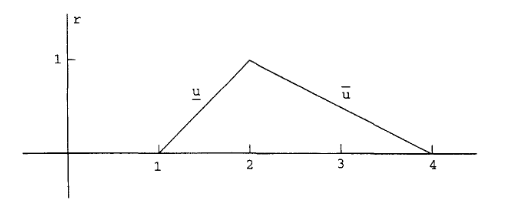
\includegraphics[width=0.6\linewidth]{assets/fuzzy_num.png}
 	\caption{نمایش عدد فازی $ \left( r - 1, 2 - \frac{1}{2} r \right)$ }
	\end{figure}
 
 	\pagebreak 
 	
 	\subsection{اعداد قطعی}
 	اگر داشته باشیم 
 	$ \underline{u}\left(r\right) = \overline{u}\left(r\right) = \alpha, 0 \leq r \leq 1 $ 
 	به $ \alpha $ عددی قطعی \LTRfootnote{crisp} گفته می شود. 
	\subsection{دستگاه فازی}
	
	دستگاه خطی $ n \times n $ زیر 
	\begin{equation}
	\label{eq:1}
	\begin{split}
	 a_{11}x_1 + a_{12}x_2 + \ldots + a_{1n}x_n = y_1 \\
	 a_{21}x_1 + a_{22}x_2 + \ldots + a_{2n}x_n = y_2 \\
	\vdots\\
	 a_{n1}x_1 + a_{n2}x_2 + \ldots + a_{nn}x_n = y_n 
	\end{split}
	\end{equation}
	که ماتریس ضرایب آن 
	$ A = \left(a_{ij}\right), 1 \leq i, j \leq n$ 
	یک ماتریس با درایه های قطعی و $ y $ برداری با اعضای فازی است را یک دستگاه خطی فازی \LTRfootnote{fuzzy linear system(FLS)} گفته می شود. \\
	به بردار فازی\LTRfootnote{fuzzy number vector}
	$ \left(x_1, x_2, \ldots, x_n\right)^T $
	که
	$ , x_i = \left(\underline{x}_i\left(r\right), \overline{x}_i\left(r\right)\right), $
	$ 1 \leq i \leq n, 0 \leq r \leq 1 $ 

	جواب دستگاه فازی گفته می شود اگر در شروط زیر صدق کند 
	\begin{equation}
	\label{eq:2}
	\begin{split}
		\overline{\sum_{i=0}^{n}a_{ij}x_j} = \sum_{i=0}^{n} a_{ij}\overline{x_j} = \overline{y_i}  \\
		\underline{\sum_{i=0}^{n}a_{ij}x_j} = \sum_{i=0}^{n} a_{ij}\underline{x_j} = \underline{y_i}
	\end{split} 
	\end{equation}    
	
	
	\subsection{جواب دستگاه فازی} 
	
	اگر 
	$ X = \lbrace\left(\underline{x}_i, -\overline{x}_i\right), 1 \leq i \leq n\rbrace $ 
	جواب یکتا دستگاه \ref{eq:8} باشد،‌ بردار فازی\\ 
	$ u = \lbrace\left(\underline{u}_i, \overline{u}_i\right), 1 \leq i \leq n\rbrace $ 
	که به صورت 
	\begin{align} 
	\underline{u}_i(r) & = \min\lbrace\underline{x}_i(r), \overline{x}_i(r), \underline{x}_i(1)\rbrace \\
	\overline{u}_i(r)  & = \max\lbrace\underline{x}_i(r), \overline{x}_i(r), \underline{x}_i(1)\rbrace
	\end{align}
	تعریف می شود، یک جواب فازی\LTRfootnote{fuzzy solution} دستگاه $ SX = Y $ می نامیم. با توجه به تعریف بالا اگر 
	$ \left(\underline{x}_i, \overline{x}_i\right) $ 
	اعداد فازی باشند، به راحتی می توان دید که 
	$ \underline{u}_i = \underline{x}_i $ 
	و 
	$ \overline{u}_i = \overline{x}_i $ 
	.در این حالت به $ U $ جواب فازی قوی \LTRfootnote{strong fuzzy solution} و در غیر اینضورت جوا ب فازی ضعیف \LTRfootnote{weak fuzzy           solution} گفته می شود. 
